\documentclass{article}
\usepackage{amsmath, sfmath, multicol, tkz-euclide, array, enumerate, tcolorbox, tabularray}
\renewcommand{\familydefault}{\sfdefault}
\setlength{\parindent}{0cm}
\pagestyle{empty}
\usepackage[left=1in, top=0.5in, right=1in, bottom=0.5in]{geometry}
\tikzset{>=stealth}
\tcbset{colback=white}

\newcounter{example}[section]
\newenvironment{example}[1][]{\refstepcounter{example}\par\medskip
   {\color{red}\textbf{Example~\theexample. #1}}}{\medskip}

\begin{document}

\section*{Reflections}

\begin{tcolorbox}[colframe=orange!70!white, coltitle=black, title=\textbf{Today I Can}]
\begin{enumerate}
    \item Find images of reflected pre-images.
\end{enumerate}
\end{tcolorbox}
\bigskip 

When reflecting across a line, count how many spaces each point is from the line.
\newline

Then count beyond the line that many spaces.
\newline

\begin{example}
Reflect each of the following. Then list the coordinates of the image.
\begin{multicols}{2}
\begin{enumerate}[(a)]
    \item Reflect across the $y$-axis  
    \item Reflect across the $x$-axis
\end{enumerate}
\end{multicols}
\begin{minipage}{0.5\textwidth}
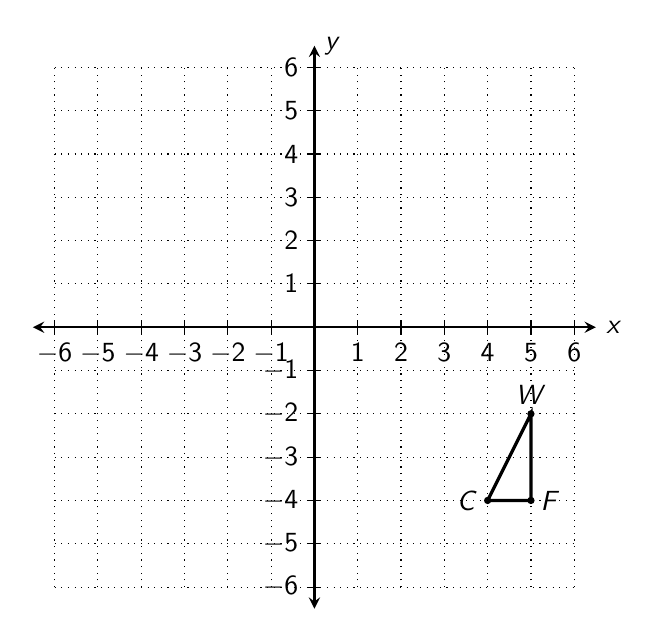
\begin{tikzpicture}[scale=0.55]
\draw[<->, thick] (-6.5,0) -- (6.5,0) node [right] {$x$};
\draw[<->, thick] (0,-6.5) -- (0,6.5) node [right] {$y$};
\draw[dotted] (-6,-6) grid (6,6);
\foreach \x in {-6,...,-1,,1,...,6}
\draw (\x, 0.15) -- (\x,-0.15) node [below] {$\footnotesize \x$};
\foreach \y in {-6,...,-1,,1,...,6}
\draw (0.15,\y) -- (-0.15,\y) node [left] {$\footnotesize \y$};
\coordinate (W) at (5,-2);
\coordinate (F) at (5,-4);
\coordinate (C) at (4,-4);
\draw[fill=black] (W) circle (2pt);
\draw[fill=black] (F) circle (2pt);
\draw[fill=black] (C) circle (2pt);
\node at (W) [anchor = south] {$W$};
\node at (F) [anchor = west] {$F$};
\node at (C) [anchor = east] {$C$};
\draw [very thick] (W) -- (F) -- (C) -- cycle;
\end{tikzpicture}
\end{minipage}
\begin{minipage}{0.4\textwidth}
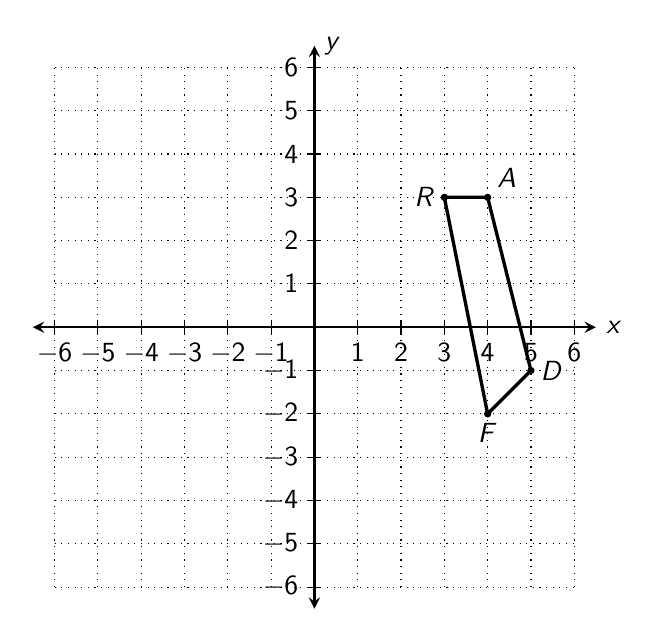
\begin{tikzpicture}[scale=0.55]
\draw[<->, thick] (-6.5,0) -- (6.5,0) node [right] {$x$};
\draw[<->, thick] (0,-6.5) -- (0,6.5) node [right] {$y$};
\draw[dotted] (-6,-6) grid (6,6);
\foreach \x in {-6,...,-1,,1,...,6}
\draw (\x, 0.15) -- (\x,-0.15) node [below] {$\tiny \x$};
\foreach \y in {-6,...,-1,,1,...,6}
\draw (0.15,\y) -- (-0.15,\y) node [left] {$\tiny \y$};
\coordinate (A) at (4,3);
\coordinate (R) at (3,3);
\coordinate (F) at (4,-2);
\coordinate (D) at (5,-1);
\draw[fill=black] (A) circle (2pt);
\draw[fill=black] (R) circle (2pt);
\draw[fill=black] (F) circle (2pt);
\draw[fill=black] (D) circle (2pt);
\node at (A) [anchor = south west] {$A$};
\node at (R) [anchor = east] {$R$};
\node at (F) [anchor = north] {$F$};
\node at (D) [anchor = west] {$D$};
\draw [very thick] (A) -- (R) -- (F) -- (D) -- cycle;
\end{tikzpicture}
\end{minipage}
\vfill 

\begin{multicols}{2}
\begin{enumerate}[(a)] \setcounter{enumi}{2}
    \item Reflect across $y = 1$
    \item Reflect across $y = x$
\end{enumerate}
\end{multicols}
\begin{minipage}{0.5\textwidth}
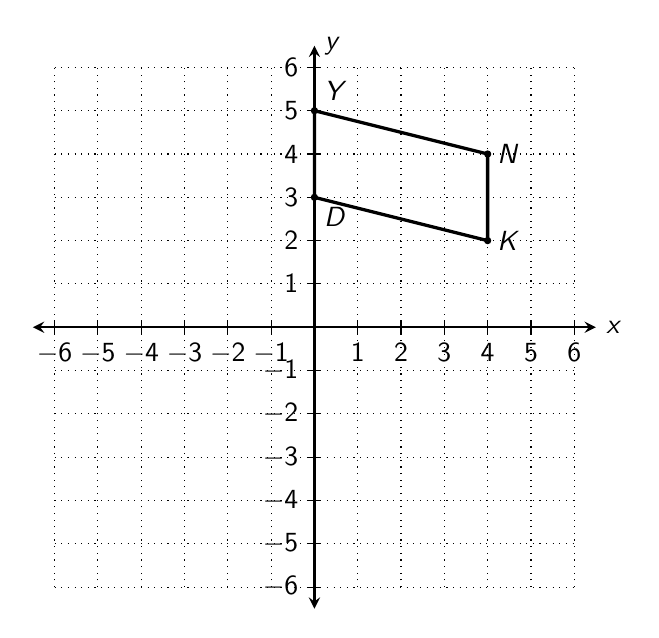
\begin{tikzpicture}[scale=0.55]
\draw[<->, thick] (-6.5,0) -- (6.5,0) node [right] {$x$};
\draw[<->, thick] (0,-6.5) -- (0,6.5) node [right] {$y$};
\draw[dotted] (-6,-6) grid (6,6);
\foreach \x in {-6,...,-1,,1,...,6}
\draw (\x, 0.15) -- (\x,-0.15) node [below] {$\tiny \x$};
\foreach \y in {-6,...,-1,,1,...,6}
\draw (0.15,\y) -- (-0.15,\y) node [left] {$\tiny \y$};
\coordinate (D) at (0,3);
\coordinate (Y) at (0,5);
\coordinate (N) at (4,4);
\coordinate (K) at (4,2);
\draw[fill=black] (D) circle (2pt);
\draw[fill=black] (K) circle (2pt);
\draw[fill=black] (N) circle (2pt);
\draw[fill=black] (Y) circle (2pt);
\node at (D) [anchor = north west] {$D$};
\node at (Y) [anchor = south west] {$Y$};
\node at (N) [anchor = west] {$N$};
\node at (K) [anchor = west] {$K$};
\draw[very thick] (D) -- (Y) -- (N) -- (K) -- cycle;
\end{tikzpicture}
\end{minipage}
\begin{minipage}{0.4\textwidth}
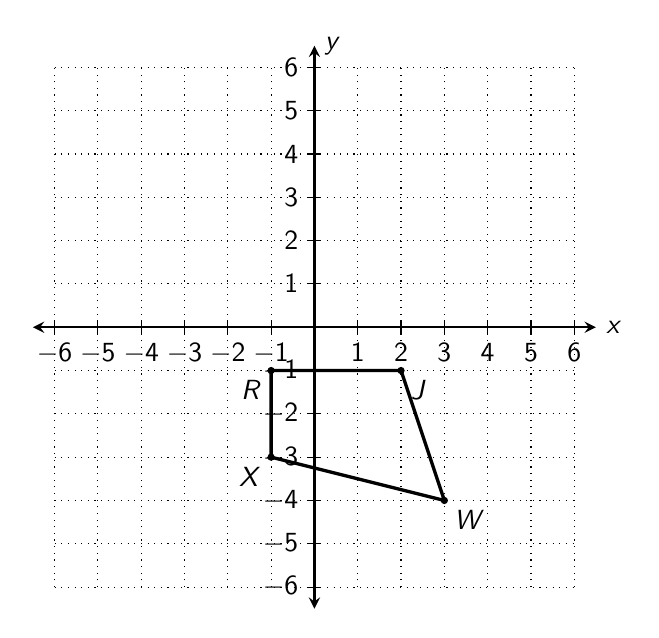
\begin{tikzpicture}[scale=0.55]
\draw[<->, thick] (-6.5,0) -- (6.5,0) node [right] {$x$};
\draw[<->, thick] (0,-6.5) -- (0,6.5) node [right] {$y$};
\draw[dotted] (-6,-6) grid (6,6);
\foreach \x in {-6,...,-1,,1,...,6}
\draw (\x, 0.15) -- (\x,-0.15) node [below] {$\tiny \x$};
\foreach \y in {-6,...,-1,,1,...,6}
\draw (0.15,\y) -- (-0.15,\y) node [left] {$\tiny \y$};
\coordinate (R) at (-1,-1);
\coordinate (X) at (-1,-3);
\coordinate (W) at (3,-4);
\coordinate (J) at (2,-1);
\draw[fill=black] (R) circle (2pt);
\draw[fill=black] (X) circle (2pt);
\draw[fill=black] (W) circle (2pt);
\draw[fill=black] (J) circle (2pt);
\node at (R) [anchor = north east] {$R$};
\node at (X) [anchor = north east] {$X$};
\node at (W) [anchor = north west] {$W$};
\node at (J) [anchor = north west] {$J$};
\draw[very thick] (R) -- (X) -- (W) -- (J) -- cycle;
\end{tikzpicture}
\end{minipage}
\end{example}

\vspace{0.25in}

\end{document}
